\documentclass[11pt,]{article}
\usepackage{lmodern}
\usepackage{amssymb,amsmath}
\usepackage{ifxetex,ifluatex}
\usepackage{fixltx2e} % provides \textsubscript
\ifnum 0\ifxetex 1\fi\ifluatex 1\fi=0 % if pdftex
  \usepackage[T1]{fontenc}
  \usepackage[utf8]{inputenc}
\else % if luatex or xelatex
  \ifxetex
    \usepackage{mathspec}
  \else
    \usepackage{fontspec}
  \fi
  \defaultfontfeatures{Ligatures=TeX,Scale=MatchLowercase}
\fi
% use upquote if available, for straight quotes in verbatim environments
\IfFileExists{upquote.sty}{\usepackage{upquote}}{}
% use microtype if available
\IfFileExists{microtype.sty}{%
\usepackage{microtype}
\UseMicrotypeSet[protrusion]{basicmath} % disable protrusion for tt fonts
}{}
\usepackage[margin=1.0in]{geometry}
\usepackage{hyperref}
\hypersetup{unicode=true,
            pdfborder={0 0 0},
            breaklinks=true}
\urlstyle{same}  % don't use monospace font for urls
\usepackage{graphicx,grffile}
\makeatletter
\def\maxwidth{\ifdim\Gin@nat@width>\linewidth\linewidth\else\Gin@nat@width\fi}
\def\maxheight{\ifdim\Gin@nat@height>\textheight\textheight\else\Gin@nat@height\fi}
\makeatother
% Scale images if necessary, so that they will not overflow the page
% margins by default, and it is still possible to overwrite the defaults
% using explicit options in \includegraphics[width, height, ...]{}
\setkeys{Gin}{width=\maxwidth,height=\maxheight,keepaspectratio}
\IfFileExists{parskip.sty}{%
\usepackage{parskip}
}{% else
\setlength{\parindent}{0pt}
\setlength{\parskip}{6pt plus 2pt minus 1pt}
}
\setlength{\emergencystretch}{3em}  % prevent overfull lines
\providecommand{\tightlist}{%
  \setlength{\itemsep}{0pt}\setlength{\parskip}{0pt}}
\setcounter{secnumdepth}{0}
% Redefines (sub)paragraphs to behave more like sections
\ifx\paragraph\undefined\else
\let\oldparagraph\paragraph
\renewcommand{\paragraph}[1]{\oldparagraph{#1}\mbox{}}
\fi
\ifx\subparagraph\undefined\else
\let\oldsubparagraph\subparagraph
\renewcommand{\subparagraph}[1]{\oldsubparagraph{#1}\mbox{}}
\fi

%%% Use protect on footnotes to avoid problems with footnotes in titles
\let\rmarkdownfootnote\footnote%
\def\footnote{\protect\rmarkdownfootnote}

%%% Change title format to be more compact
\usepackage{titling}

% Create subtitle command for use in maketitle
\newcommand{\subtitle}[1]{
  \posttitle{
    \begin{center}\large#1\end{center}
    }
}

\setlength{\droptitle}{-2em}

  \title{}
    \pretitle{\vspace{\droptitle}}
  \posttitle{}
    \author{}
    \preauthor{}\postauthor{}
    \date{}
    \predate{}\postdate{}
  
\usepackage{helvet} % Helvetica font
\renewcommand*\familydefault{\sfdefault} % Use the sans serif version of the font
\usepackage[T1]{fontenc}

\usepackage[none]{hyphenat}

\usepackage{setspace}
\doublespacing
\setlength{\parskip}{1em}

\usepackage{lineno}

\usepackage{pdfpages}

\begin{document}

\vspace{35mm}

\section{\texorpdfstring{The proton pump inhibitor omeprazole does not
promote \emph{Clostridium difficile} colonization in a murine
model}{The proton pump inhibitor omeprazole does not promote Clostridium difficile colonization in a murine model}}\label{the-proton-pump-inhibitor-omeprazole-does-not-promote-clostridium-difficile-colonization-in-a-murine-model}

\vspace{35mm}

Sarah Tomkovich\({^1}\), Nicholas A. Lesniak\({^1}\), Yuan Li\({^1}\),
Lucas Bishop\({^1}\), Madison J. Fitzgerald\({^1}\), Patrick D.
Schloss\textsuperscript{1\(\dagger\)}

\vspace{40mm}

\(\dagger\) To whom correspondence should be addressed:
\href{mailto:pschloss@umich.edu}{\nolinkurl{pschloss@umich.edu}}

\(1\) Department of Microbiology and Immunology, University of Michigan,
Ann Arbor, MI 48109

\newpage

\linenumbers

\subsection{Abstract}\label{abstract}

Proton pump inhibitor (PPI) use has been associated with microbiota
alterations and susceptibility to \emph{Clostridium}
(\emph{Clostridioides}) \emph{difficile} infections (CDIs) in humans. We
assessed how PPI treatment alters the fecal microbiota and whether
treatment promotes CDIs in a mouse model. Mice receiving a PPI treatment
were gavaged with 40 mg/kg of omeprazole during a 7-day pretreatment
phase, the day of \emph{C. difficile} challenge, and the following 9
days. We found that mice treated with omeprazole were not colonized by
\emph{C. difficile}. When omeprazole treatment was combined with a
single clindamycin treatment, one cage of mice remained resistant to
\emph{C. difficile} colonization, while the other cage was colonized.
Treating mice with only clindamycin followed by challenge resulted in
\emph{C. difficile} colonization. 16S rRNA gene sequencing analysis
revealed that omeprazole had minimal impact on the structure of the
murine microbiota throughout the 16 days of omeprazole exposure. These
results suggest omeprazole treatment alone is not sufficient to disrupt
microbiota resistance to \emph{C. difficile} infection in mice that are
normally resistant in the absence of antibiotic treatment.

\subsection{Importance}\label{importance}

Antibiotics are the primary risk factor for \emph{Clostridium}
(\emph{Clostridioides}) \emph{difficile} infections (CDIs), but other
factors may also increase a person's risk. In epidemiological studies,
proton pump inhibitor (PPI) use has been associated with CDI incidence
and recurrence. PPIs have also been associated with alterations in the
human intestinal microbiota in observational and interventional studies.
We evaluated the effects of the PPI omeprazole on the structure of the
murine intestinal microbiota and its ability to disrupt colonization
resistance to \emph{C. difficile}. We found omeprazole treatment had
minimal impact on the murine fecal microbiota and did not promote
\emph{C. difficile} colonization. Further studies are needed to
determine whether other factors contribute to the association between
PPIs and CDIs seen in humans or whether aspects of murine physiology may
limit its utility to test these types of hypotheses.

\newpage

Antibiotics have a large impact on the intestinal microbiome and are a
primary risk factor for developing \emph{Clostridium}
(\emph{Clostridioides}) \emph{difficile} infections (CDIs) (1). It is
less clear whether other human medications that impact the microbiota
also influence \emph{C. difficile} colonization resistance. Multiple
epidemiological studies have suggested an association between proton
pump inhibitor (PPI) use and incidence or recurrence of CDIs (2--5).
There have also been a number of large cohort studies and interventional
clinical trials that demonstrated specific alterations in the intestinal
microbiome were associated with PPI use (4, 6). PPI-associated
microbiota changes have been attributed to the ability of PPIs to
increase stomach acid pH which may promote the survival of oral and
pathogenic bacteria (4, 6). In human fecal samples, PPI use results in
increases in \emph{Enterococcaceae}, \emph{Lactobacillaceae},
\emph{Micrococcaceae}, \emph{Staphylococcaceae} and
\emph{Streptococcaceae} and decreases in \emph{Ruminococcaceae} (6--9).
Several of these taxa have also been associated with \emph{C. difficile}
colonization in humans (10).\\
Unfortunately, the studies suggesting a link between PPIs and \emph{C.
difficile} were retrospective and did not evaluate changes in the
microbiome (2, 3, 5). Thus, it is unclear whether the gastrointestinal
microbiome changes associated with PPI use explain the association
between PPIs and CDIs. Additionally, epidemiological studies have a
limited capacity to address potential confounders and comorbidities in
patients that were on PPIs and developed CDIs or recurrent CDIs (2, 5).
Here, we evaluated the impact of daily PPI treatment with omeprazole on
the murine microbiome and susceptibility to \emph{C. difficile}
colonization in relation to clindamycin, an antibiotic that perturbs the
microbiome enough to allow \emph{C. difficile} to colonize but is mild
enough that \emph{C. difficile} is cleared within 10 days (11).

\textbf{Murine fecal microbiomes were minimally affected by omeprazole
treatment. } To test whether omeprazole treatment alters the microbiome
and promotes susceptibility to CDIs, we gavaged mice with 40 mg/kg of
omeprazole for 7 days before \emph{C. difficile} challenge (Figure 1A).
A principle coordinates analysis (PCoA) of the Bray-Curtis distances
over the initial 7 days of treatment revealed the bacterial communities
of omeprazole-treated mice remained relatively unchanged (Figure 1B). We
observed no significant changes in the relative abundance of those taxa
previously shown to respond to PPI treatment throughout the course of
the 16-day experiment (Figure 1C-D, S1). We also observed no significant
changes in relative abundances at the family and genus level over the
course of the experiment for the omeprazole-treated mice (all corrected
P-values \textgreater{} 0.36). These results demonstrated that the
omeprazole treatment alone had a minimal impact on the murine fecal
bacterial community after 7 days of pretreatment.

\textbf{Omeprazole treatment did not promote susceptibility to \emph{C.
difficile} infection in mice.} Next, we examined whether omeprazole
treatment altered susceptibility to \emph{C. difficile} infection in
mice. After omeprazole treatment or clindamycin treatment, mice were
challenged with 10\textsuperscript{3} \emph{C. difficile} 630 spores.
Although \emph{C. difficile} colonized the clindamycin-treated mice, it
did not colonize the omeprazole-treated mice (Figure 2A). Interestingly,
only 1 cage of mice that received both omeprazole and clindamycin were
colonized, while the other cage of mice were resistant (Figure 2A). The
greatest shifts in bacterial communities occurred in the
clindamycin-treated mice (Figure 2B, S2). Regardless of whether the mice
became colonized, all of the mice had cleared \emph{C. difficile} within
5 days (Figure 2A), suggesting that omeprazole did not affect the rate
of clearance. Our results suggest that omeprazole treatment had no
effect on bacterial community resistance to \emph{C. difficile}
colonization in mice. Instead most of the differences between the 3
treatment groups appeared to be driven by clindamycin administration
(Figure 2C, S2). These findings demonstrated that high dose omeprazole
treatment did not promote susceptibility to \emph{C. difficile}
colonization.

\textbf{Conclusions.} The PPI omeprazole did not meaningfully impact the
structure of the gut microbiota and did not promote \emph{C. difficile}
infection in mice. Our findings that omeprazole treatment had minimal
impact on the fecal microbiome were comparable to another PPI mouse
study that indicated the PPI lansoprazole had more of an effect on the
small intestinal microbiota compared to the fecal microbiota (12). The
same group demonstrated lansoprazole treatment increased the stomach pH
in mice (12), which may improve survival of bacteria passing through the
stomach. We did not find significant changes in the relative abundances
of the taxa observed to be significantly impacted by PPI use in human
studies. However, 3 of the human-associated taxa were absent or at low
abundance in our mice. Interestingly, other groups examining fecal
microbiota communities before and after PPI administration to healthy
cats and infants with gastroesophageal reflux disease, found PPIs have
minimal effects on fecal bacterial community structures, although there
were a few significant changes in specific genera (13, 14). One
limitation of our study is that there were only 4-5 mice per group,
which may have limited our ability to identify PPI-induced changes in
specific bacteria genera. Although our fecal microbiota findings are
comparable to what has been shown in another mouse study (12), whether
PPI-induced changes in specific bacterial abundances observed in humans
play a role in CDIs remains to be determined.\\
Although several \emph{C. difficile} mouse model studies have shown that
PPIs have an effect on CDIs with or without additional antibiotic
treatment (15--17), there were insufficient controls to attribute the
effect solely to PPI treatment. One group administered 0.5 mg/kg of the
PPI lansoprazole daily for 2 weeks to mice and then challenged with
\emph{C. difficile} demonstrated that PPI treatment alone resulted in
detectable \emph{C. difficile} in the stool 1 week after challenge,
however there was detectable \emph{C. difficile} in mice not treated
with antibiotics (15, 16). The other mouse study demonstrated
antibiotic/esomeprazole-treated mice developed more severe CDIs compared
to antibiotic-treated mice, but the researchers did not have a group
treated with just esomeprazole for comparison (17). We tested the same
high 40 mg/kg PPI dose and expanded pre-treatment to 7 days before
challenge to test the impact of omeprazole treatment alone on our CDI
mouse model. Additionally, we have previously demonstrated that mice
from our breeding colony are resistant to \emph{C. difficile} 630
colonization without antibiotic treatment (18), ensuring there was not
already partial susceptibility to \emph{C. difficile} before treatment.
The additional controls in our study allowed us to assess the
contribution of omeprazole alone to \emph{C. difficile} susceptibility
in mice.\\
Our study also extended previous work examining PPIs and \emph{C.
difficile} in mice by incorporating the contribution of the intestinal
microbiota. We found omeprazole had no significant impact on bacterial
taxa within the murine intestinal microbiota over the 16-day experiment.
In contrast to previous work with PPIs (15--17), omeprazole did not
alter \emph{C. difficile} colonization resistance in mice. 16S rRNA
sequencing suggested that \emph{Streptococcus} and \emph{Enterococcus}
are rare genera in our C57BL/6 mouse colony. These two genera could be
important contributors to the associations between PPIs and CDIs in
humans, and could be a contributing factor to our observation that PPI
treatment had no effect on \emph{C. difficile} colonization in our CDI
mouse model. While the intestinal microbiomes of both humans and mice
are dominated by the \emph{Bacteroidetes} and \emph{Firmicutes} phyla,
there are significant differences in the relative abundances of genera
that are present and some genera are unique to each mammal (19),
differences that may partly explain our results. Gastrointestinal
physiological differences, particularly the higher stomach pH in mice
(pH 3-4) compared to humans (pH 1) (19) could also explain why
omeprazole had a limited impact on the murine microbiome. The microbiota
and physiological differences between humans and mice may limit the
usefulness of employing mouse models to study the impact of PPIs on the
microbiota and CDIs.\\
Beyond microbiome differences, factors such as age, body mass index,
comorbidities, and use of other medications in human studies may also be
contributing to the association between PPIs and CDI incidence or
recurrence. The type of \emph{C. difficile} strain type could also be an
important contributing factor, however our study was limited in that we
only tested \emph{C. difficile} 630 (ribotype 012). This study addressed
the impact of PPIs with or without antibiotics on a murine model of CDI,
and found PPIs did not promote \emph{C. difficile} colonization. The
epidemiological evidence linking PPIs to CDIs is primarily from
observational studies, which makes determining causality and whether
other risk factors play a role challenging (20). Future studies are
needed to determine whether age, other comorbidities and bacterial
strains that are less common in mice can increase the risk of CDIs or
recurrent CDIs when combined with PPI treatment.

\subsection{Acknowledgements}\label{acknowledgements}

This research was supported by NIH grant U01AI12455. We would also like
to thank the Unit for Laboratory Animal Medicine at the University of
Michigan for maintaining our mouse colony and providing the
infrastructure and support for performing our mouse experiments. The
authors are also thankful to members of the Schloss lab for helpful
discussions throughout the process of designing the experiment,
analyzing the results, crafting the figures, and drafting of the
manuscript.

\newpage

\subsection{Materials and Methods}\label{materials-and-methods}

\textbf{Animals.} All mouse experiments were performed with 7- to
12-week-old C57BL/6 male and female mice. Each experimental group of
mice was split between 2 cages with 2-3 mice housed per cage and male
and female mice housed separately. All animal experiments were approved
by the University of Michigan Animal Care and Use Committee (IACUC)
under protocol number PRO00006983.

\textbf{Drug treatments.} Omeprazole (Sigma Aldrich) was prepared in a
vehicle solution of 40\% polyethylene glycol 400 (Sigma-Aldrich) in
phosphate buffered saline. Omeprazole was prepared from 20 mg/mL frozen
aliquots and diluted to an 8 mg/mL prior to gavage. All mice received 40
mg/kg omeprazole (a dose previously used in mouse experiments (17)) or
vehicle solution once per day through the duration of the experiment
with treatment starting 7 days before \emph{C. difficile} challenge
(Figure 1A). Although the omeprazole dose administered to mice is higher
than the recommended dose for humans, omeprazole has a shorter half-life
in mice compared to humans (21) and lacks an enteric coating (22). One
day prior to \emph{C. difficile} challenge, 2 groups of mice received an
intraperitoneal injection of 10 mg/kg clindamycin or sterile saline
vehicle (11). All drugs were filter sterilized through a 0.22 micron
syringe filter before administration to animals.

\textbf{\emph{C. difficile} infection model.} Mice were challenged with
\emph{C. difficile} 630 seven days after the start of omeprazole
treatment and one day after clindamycin treatment. Mice were challenged
with 10\textsuperscript{3} spores in ultrapure distilled water as
described previously (11). Stool samples were collected for 16S rRNA
sequencing or \emph{C. difficile} CFU quantification throughout the
duration of the experiments at the indicated timepoints (Figure 1A).
Samples for 16S rRNA sequencing were flash frozen in liquid nitrogen and
stored at -80°C until DNA extraction, while samples for CFU
quantification were transferred into an anaerobic chamber and serially
diluted in PBS. Diluted samples were plated on TCCFA (taurocholate,
cycloserine, cefoxitin, fructose agar) plates and incubated at 37°C for
24 hours under anaerobic conditions to quantify \emph{C. difficile} CFU.

\textbf{16S rRNA gene sequencing.} DNA for 16S rRNA gene sequencing was
extracted from 10-50 mg fecal pellet from each mouse using the DNeasy
Powersoil HTP 96 Kit (Qiagen) and an EpMotion 5075 automated pipetting
system (Eppendorf). The 16S rRNA sequencing library was prepared as
described previously (23). In brief, the ZymoBIOMICS\textsuperscript{TM}
Microbial Community DNA Standard (Zymo, CA, USA) was used as a mock
community (24) and water was used as a negative control. The V4
hypervariable region of the 16S rRNA gene was amplified with Accuprime
Pfx DNA polymerase (Thermo Fisher Scientific) using previously described
custom barcoded primers (23). The 16S rRNA amplicon library was
sequenced with the MiSeq (Illumina). Amplicons were cleaned up and
normalized with the SequalPrep Normalization Plate Kit (ThermoFisher
Scientific) and pooled amplicons were quantified with the KAPA library
quantification kit (KAPA Biosystems).

\textbf{16S rRNA gene sequence analysis.} mothur (v1.40.5) was used for
all sequence processing steps (25) using a previously published protocol
(23). In brief, forward and reverse reads for each sample were combined
and low-quality sequences and chimeras were removed. Duplicate sequences
were merged, before taxonomy assignment using a modified version (v16)
of the Ribosomal Database Project reference database (v11.5) with an
80\% cutoff. Operational taxonomic units (OTUs) were assigned with the
opticlust clustering algorithm using a 97\% similarity threshold. To
adjust for uneven sequencing across samples, all samples were rarefied
to 3,000 sequences, 1,000 times. PCoAs were generated based on
Bray-Curtis distance. R (v.3.5.1) was used to generate figures and
perform statistical analysis.

\textbf{Statistical Analysis.} To test for differences in relative
abundances in families and genera across our 3 different treatment
groups at different timepoints (Clindamycin, Clindamycin + Omeprazole,
and Omeprazole on Day -7, 0, 2, and 9) or within the Omeprazole
treatment group across 3 timepoints (Day -7, 0, and 9), we used a
Kruskal-Wallis test with a Benjamini-Hochberg correction for multiple
comparisons.

\textbf{Code availability.} The code for all sequence processing and
analysis steps as well as a Rmarkdown version of this manuscript is
available at
\url{https://github.com/SchlossLab/Tomkovich_PPI_mSphere_2019}.

\textbf{Data availability.} The 16S rRNA sequencing data have been
deposited in the NCBI Sequence Read Archive (Accession no. PRJNA554866).

\newpage

\subsection{References}\label{references}

\hypertarget{refs}{}
\hypertarget{ref-Schubert2015}{}
1. Schubert AM, Sinani H, Schloss PD. 2015. Antibiotic-induced
alterations of the murine gut microbiota and subsequent effects on
colonization resistance against \emph{Clostridium difficile}. mBio 6.

\hypertarget{ref-tariq2017association}{}
2. Tariq R, Singh S, Gupta A, Pardi DS, Khanna S. 2017. Association of
gastric acid suppression with recurrent \emph{Clostridium difficile}
infection: A systematic review and meta-analysis. JAMA internal medicine
177:784--791.

\hypertarget{ref-nehra2018proton}{}
3. Nehra AK, Alexander JA, Loftus CG, Nehra V. 2018. Proton pump
inhibitors: Review of emerging concerns, pp. 240--246. \emph{In} Mayo
clinic proceedings. Elsevier.

\hypertarget{ref-Naito2018}{}
4. Naito Y, Kashiwagi K, Takagi T, Andoh A, Inoue R. 2018. Intestinal
dysbiosis secondary to proton-pump inhibitor use. Digestion 97:195--204.

\hypertarget{ref-Elias2019}{}
5. Elias E, Targownik LE. 2019. The clinician's guide to proton pump
inhibitor related adverse events. Drugs 79:715--731.

\hypertarget{ref-Imhann2017}{}
6. Imhann F, Vila AV, Bonder MJ, Manosalva AGL, Koonen DP, Fu J,
Wijmenga C, Zhernakova A, Weersma RK. 2017. The influence of proton pump
inhibitors and other commonly used medication on the gut microbiota. Gut
Microbes 8:351--358.

\hypertarget{ref-Imhann2015}{}
7. Imhann F, Bonder MJ, Vila AV, Fu J, Mujagic Z, Vork L, Tigchelaar EF,
Jankipersadsing SA, Cenit MC, Harmsen HJM, Dijkstra G, Franke L, Xavier
RJ, Jonkers D, Wijmenga C, Weersma RK, Zhernakova A. 2015. Proton pump
inhibitors affect the gut microbiome. Gut 65:740--748.

\hypertarget{ref-Freedberg2015}{}
8. Freedberg DE, Toussaint NC, Chen SP, Ratner AJ, Whittier S, Wang TC,
Wang HH, Abrams JA. 2015. Proton pump inhibitors alter specific taxa in
the human gastrointestinal microbiome: A crossover trial.
Gastroenterology 149:883--885.e9.

\hypertarget{ref-maier2018extensive}{}
9. Maier L, Pruteanu M, Kuhn M, Zeller G, Telzerow A, Anderson EE,
Brochado AR, Fernandez KC, Dose H, Mori H, others. 2018. Extensive
impact of non-antibiotic drugs on human gut bacteria. Nature 555:623.

\hypertarget{ref-Schuberte01021-14}{}
10. Schubert AM, Rogers MAM, Ring C, Mogle J, Petrosino JP, Young VB,
Aronoff DM, Schloss PD. 2014. Microbiome data distinguish patients with
\emph{Clostridium difficile} infection and non-\emph{C.
difficile}-associated diarrhea from healthy controls. mBio 5.

\hypertarget{ref-Jenior2018}{}
11. Jenior ML, Leslie JL, Young VB, Schloss PD. 2018. \emph{Clostridium
difficile} alters the structure and metabolism of distinct cecal
microbiomes during initial infection to promote sustained colonization.
mSphere 3.

\hypertarget{ref-Yasutomi2018}{}
12. Yasutomi E, Hoshi N, Adachi S, Otsuka T, Kong L, Ku Y, Yamairi H,
Inoue J, Ishida T, Watanabe D, Ooi M, Yoshida M, Tsukimi T, Fukuda S,
Azuma T. 2018. Proton pump inhibitors increase the susceptibility of
mice to oral infection with enteropathogenic bacteria. Digestive
Diseases and Sciences 63:881--889.

\hypertarget{ref-Schmid2018}{}
13. Schmid SM, Suchodolski JS, Price JM, Tolbert MK. 2018. Omeprazole
minimally alters the fecal microbial community in six cats: A pilot
study. Frontiers in Veterinary Science 5.

\hypertarget{ref-Castellani2017}{}
14. Castellani C, Singer G, Kashofer K, Huber-Zeyringer A, Flucher C,
Kaiser M, Till H. 2017. The influence of proton pump inhibitors on the
fecal microbiome of infants with gastroesophageal refluxA prospective
longitudinal interventional study. Frontiers in Cellular and Infection
Microbiology 7.

\hypertarget{ref-Kaur2007}{}
15. Kaur S, Vaishnavi C, Prasad KK, Ray P, Kochhar R. 2007. Comparative
role of antibiotic and proton pump inhibitor in experimental
\emph{Clostridium difficile} infection in mice. Microbiology and
Immunology 51:1209--1214.

\hypertarget{ref-kaur2011effect}{}
16. Kaur S, Vaishnavi C, Prasad KK, Ray P, Kochhar R. 2011. Effect of
lactobacillus acidophilus \& epidermal growth factor on experimentally
induced \emph{Clostridium difficile} infection. The Indian journal of
medical research 133:434.

\hypertarget{ref-hung2015proton}{}
17. Hung Y-P, Ko W-C, Chou P-H, Chen Y-H, Lin H-J, Liu Y-H, Tsai H-W,
Lee J-C, Tsai P-J. 2015. Proton-pump inhibitor exposure aggravates
\emph{Clostridium difficile}--associated colitis: Evidence from a mouse
model. The Journal of infectious diseases 212:654--663.

\hypertarget{ref-Jenior2017}{}
18. Jenior ML, Leslie JL, Young VB, Schloss PD. 2017. \emph{Clostridium
difficile} colonizes alternative nutrient niches during infection across
distinct murine gut microbiomes. mSystems 2.

\hypertarget{ref-Hugenholtz2018}{}
19. Hugenholtz F, Vos WM de. 2018. Mouse models for human intestinal
microbiota research: A critical evaluation. Cellular and Molecular Life
Sciences 75:149--160.

\hypertarget{ref-Eze2017}{}
20. Eze P, Balsells E, Kyaw MH, Nair H. 2017. Risk factors for
\emph{Clostridium difficile} infections -- an overview of the evidence
base and challenges in data synthesis. Journal of Global Health 7.

\hypertarget{ref-Regrdh1985}{}
21. Regårdh C-G, Gabrielsson M, Hoffman K-J, Löfberg I, Skånberg I.
1985. Pharmacokinetics and metabolism of omeprazole in animals and man -
an overview. Scandinavian Journal of Gastroenterology 20:79--94.

\hypertarget{ref-Llorente2017}{}
22. Llorente C, Jepsen P, Inamine T, Wang L, Bluemel S, Wang HJ, Loomba
R, Bajaj JS, Schubert ML, Sikaroodi M, Gillevet PM, Xu J, Kisseleva T,
Ho SB, DePew J, Du X, Sørensen HT, Vilstrup H, Nelson KE, Brenner DA,
Fouts DE, Schnabl B. 2017. Gastric acid suppression promotes alcoholic
liver disease by inducing overgrowth of intestinal enterococcus. Nature
Communications 8.

\hypertarget{ref-Kozich2013}{}
23. Kozich JJ, Westcott SL, Baxter NT, Highlander SK, Schloss PD. 2013.
Development of a dual-index sequencing strategy and curation pipeline
for analyzing amplicon sequence data on the MiSeq illumina sequencing
platform. Applied and Environmental Microbiology 79:5112--5120.

\hypertarget{ref-Sze2019}{}
24. Sze MA, Schloss PD. 2019. The impact of DNA polymerase and number of
rounds of amplification in PCR on 16S rRNA gene sequence data. mSphere
4.

\hypertarget{ref-Schloss2009}{}
25. Schloss PD, Westcott SL, Ryabin T, Hall JR, Hartmann M, Hollister
EB, Lesniewski RA, Oakley BB, Parks DH, Robinson CJ, Sahl JW, Stres B,
Thallinger GG, Horn DJV, Weber CF. 2009. Introducing mothur:
Open-source, platform-independent, community-supported software for
describing and comparing microbial communities. Applied and
Environmental Microbiology 75:7537--7541.

\newpage

\subsection{Figures}\label{figures}

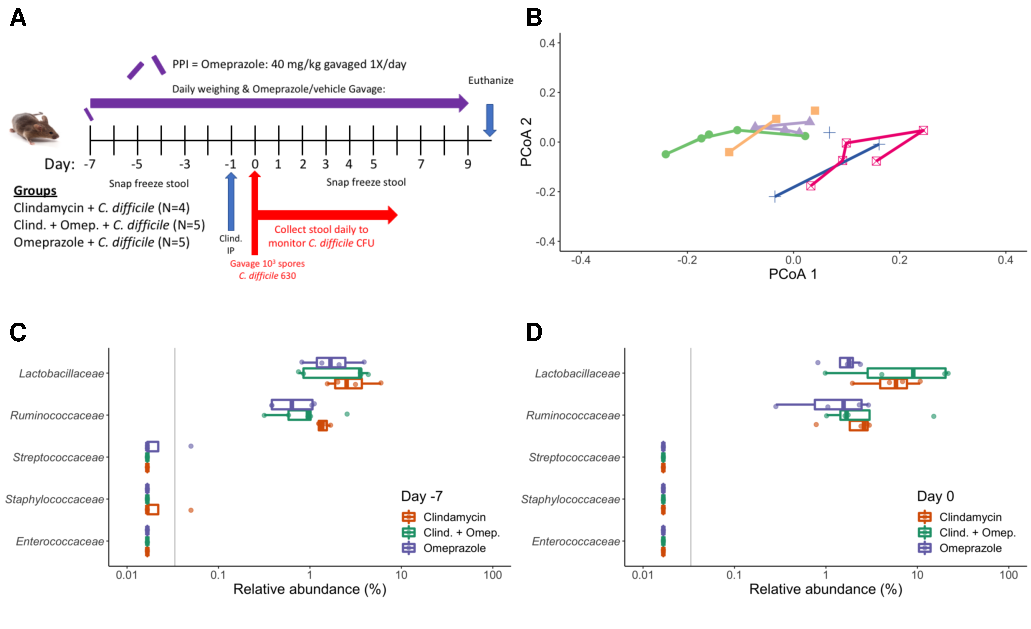
\includegraphics{figure_1.pdf} \textbf{Figure 1. Omeprazole treatment
had minimal impact on the murine fecal microbiota.} A. Mouse experiment
timeline and logistics. The PPI omeprazole was administered throughout
the duration of the experiment. Clindamycin was administered 1 day
before \emph{C. difficile} challenge on Day 0. Stools for 16S rRNA
sequencing analysis were collected on the days that are labeled (Day -7,
-5, -3, -1, 0, 1, 2, 3, 4, 5, 7, 9). \emph{C. difficile} CFU in the
stool was quantified daily through 6 days post-infection by anaerobic
culture. B. Principal Coordinates Analysis (PCoA) of Bray-Curtis
distances from stool samples of mice in the omeprazole treatment group
during the initial 7 days of the experiment. Each color represents stool
samples from the same mouse and lines connect sequentially collected
samples. C-D. Relative abundances of families previously associated with
PPI use in humans at the start of the experiment (C) and after 7 days of
omeprazole treatment (D). Each circle represents an individual mouse.
There were no significant differences across treatment groups for any of
the identified families in the sequence data at day -7 (all P-values
\textgreater{} 0.448) and day 0 (all P-values \textgreater{} 0.137),
analyzed by Kruskal-Wallis test with a Benjamini-Hochberg correction for
multiple comparisons. For C-D, the grey vertical line indicates the
limit of detection.

\newpage

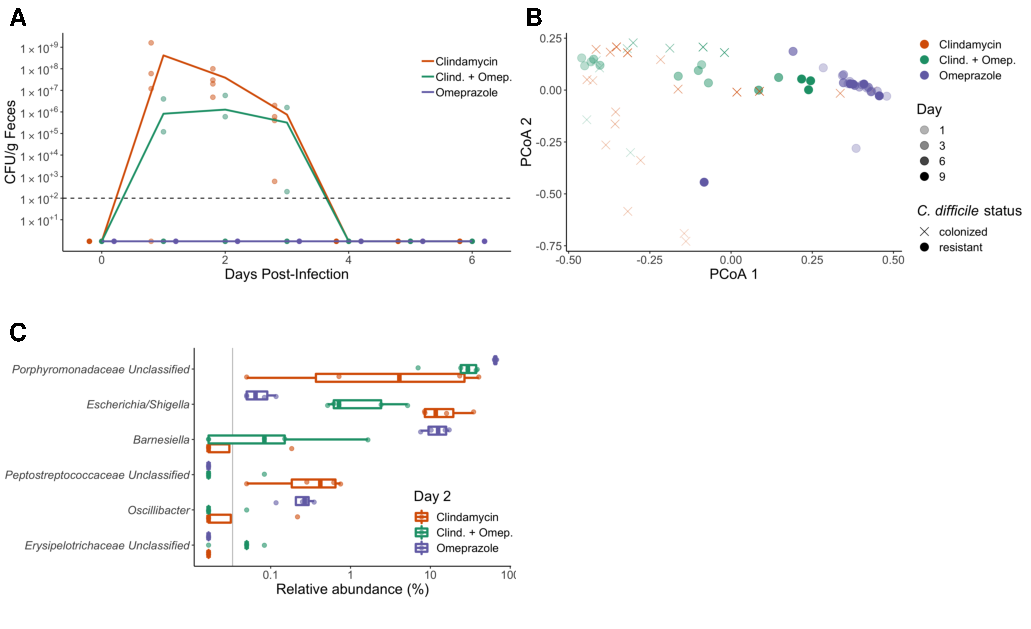
\includegraphics{figure_2.pdf} \textbf{Figure 2. Omeprazole treatment
alone does not promote CDIs in mice.} A. \emph{C. difficile} CFUs/g
stool measured each day post \emph{C. difficile} challenge for
clindamycin, clindamycin/omeprazole, and omeprazole-treated mice. Lines
represent the mean CFU/g for each treatment group while points represent
CFU/g for individual mice within each group. The black dashed line
indicates the limit of detection. B. PCoA of of Bray-Curtis distances
from stool samples collected after antibiotic treatment (last 9 days of
the experiment). Transparency of the symbol corresponds to treatment
day. Symbols represent the \emph{C. difficile} colonization status of
the mice measured 2 days post-infection. Circles represent resistant
mice (\emph{C. difficile} was undetectable in stool samples), while
X-shapes represent mice that were colonized with \emph{C. difficile},
although all mice cleared \emph{C. difficile} within 5 days of
infection. Omeprazole treated fecal samples primarily cluster together
throughout the experiment. C. Genera that vary the most across treatment
groups for stool samples collected from mice 2 days post-infection. Data
were analyzed by Kruskal-Wallis test, and no P-values were significant
after Benjamini-Hochberg correction for multiple comparisons (all
P-values \textgreater{} 0.092). The grey vertical line indicates the
limit of detection.

\newpage

\includegraphics{figure_s1.pdf} \textbf{Figure S1. Families within
omeprazole treated mice fluctuate over time with no overall trend in
either direction.} Relative abundance over time for
\emph{Lactobacillaceae} (A) and \emph{Ruminococcaceae} (B), 2 of the
PPI-associated families from human PPI studies across all 3 treatment
groups. Each point represents the relative abundance for an individual
mouse stool sample, while the lines represent the mean relative
abundances for each treatment group of mice. The grey horizontal lines
indicate the limit of detection.

\newpage

\includegraphics{figure_s2.pdf} \textbf{Figure S2. Microbiota diversity
and richness decrease with antibiotic treatment but remain relatively
constant with omeprazole treatment.} Boxplots of the Shannon Diversity
Index values (A) and number of observed OTUs (B) for each group of mice
over 3 timepoints (Day -7, 0, and 9). Each circle represents the value
for a stool sample from an individual mouse.


\end{document}
